\documentclass[12pt,a4paper,landscape]{article}
\usepackage{fontspec}
\usepackage[french]{babel}
\usepackage[utf8]{inputenc}
\usepackage[right=0.5cm, left=0.5cm,top=0.5cm,bottom=0.5cm]{geometry}
\usepackage{enumitem}
\usepackage{graphicx}
\usepackage{wrapfig}  % Package to wrap figures
\usepackage{array}
\usepackage{amsmath,amsfonts,amssymb,mathrsfs,amsthm}
\usepackage{fancyhdr}

\usepackage{rotating}%for rotating tables

\usepackage[usenames,svgnames,dvipsnames]{xcolor}
\usepackage{color}
%\mathchardef\times="2202
\definecolor{lightgray}{gray}{0.9}
\definecolor{ocre}{RGB}{0,244,244} 

\usepackage[most]{tcolorbox}
\usepackage{booktabs}
\usepackage[font={bf}]{caption}
\captionsetup[table]{box=colorbox,boxcolor=orange!20}
\usepackage{float}
\usepackage{esvect}
\usepackage{tabularx}
\usepackage{supertabular}
\usepackage{longtable}
\usepackage{colortbl}
\usepackage{fancybox}
\usepackage{tikz}
\usetikzlibrary{positioning,calc,intersections,patterns,decorations.pathmorphing,arrows.meta,decorations.markings}
\usetikzlibrary{arrows.meta}
\usepackage{ulem}
\usepackage{fontawesome5}
\usepackage{textcomp}
\usepackage{framed}
\usepackage{multicol}
\usepackage{varwidth}
\usetikzlibrary{calc}
\usepackage{pgfplots}
\usepackage{fourier}
\pgfplotsset{compat=1.11}
\usepackage{tkz-tab}
%\usepackage{xcolor}
\RequirePackage[framemethod=default]{mdframed}

\makeatletter
\tcbuselibrary{skins,breakable,xparse}
\tcbset{%
	save height/.code={%
		\tcbset{breakable}%
		\providecommand{#1}{2cm}%
		\def\tcb@split@start{%
			\tcb@breakat@init%
			\tcb@comp@h@page%
			\def\tcb@ch{%
				\tcbset{height=\tcb@h@page}%
				\tcbdimto#1{#1+\tcb@h@page-\tcb@natheight}%
				\immediate\write\@auxout{\string\gdef\string#1{#1}}%
				\tcb@ch%
			}%
			\tcb@drawcolorbox@standalone%
		}%
	}%
}

\makeatother
\newcommand{\oij}{$\left(\text{O};\vv{i},\vv{j},\vv{k}\right)$}
\colorlet{darkred}{red!30!black}
\newcommand{\red}[1]{\textcolor{darkred}{ #1}}
\newcommand{\rr}{\mathbb{R}}
\renewcommand{\baselinestretch}{1.2}
\setlength{\arrayrulewidth}{1.25pt}
\usepackage{titlesec}
\usepackage{titletoc}
\usepackage{minitoc}

%\usepackage[no-math]{fontspec}
\usepackage{polyglossia}
\makeatletter 
%\AtBeginDocument{\bidi@isloaded[]{frenchxetex}}
\makeatother
\setdefaultlanguage{french}
%\setdefaultlanguage[calendar=gregorian,locale=algeria]{arabic}
\setotherlanguage{english}
\newfontfamily\fontf[Scale=1]{Amiri-Bold.ttf} %Simplified Arabic
\newfontfamily\fontsf[Scale=1]{GE New Bold.ttf}%Aljazeera
\newfontfamily\myfont[Scale=1.3]{Bell MT}%AlBattar

%*************************************************************+
\colorlet{dlines}{orange!15!white}
\colorlet{llines}{orange!015!white}
\tikzset{
	dashed lines/.style={llines, very thin, densely dashed},
	strong lines/.style={dlines, very thin},
}
%--------------------------------------------------------------
\tcbset{
	enhanced,
	colback=white,
	boxrule=0.1pt,
	colframe=brown!10,
	fonttitle=\bfseries
}
\newcommand*{\arraycolor}[1]{\protect\leavevmode\color{#1}}
\newcolumntype{A}{>{\columncolor{blue!50!white}}c}
\newcolumntype{B}{>{\columncolor{LightGoldenrod}}c}
\newcolumntype{C}{>{\columncolor{FireBrick!50}}c}
\newcolumntype{D}{>{\columncolor{Gray!42}}c}
%------------------------------------------------
\newtcolorbox{box1}[2]{breakable,
	enhanced,
	leftrule=0pt,
	toprule=0pt,
	outer arc=0pt,
	arc=0pt,
	colframe=#2,
	colback=#2!3,title=#1,coltitle=white,
	attach boxed title to top right,
	boxed title style={
		colback=#2,
		outer arc=0pt,
		arc=0pt,
		top=3pt,
		bottom=3pt,
	},
	fonttitle= \bfseries}
\newtcolorbox{box2}[2]{enhanced,breakable,pad at break*=1mm,skin=enhancedlast jigsaw,
	attach boxed title to top right={xshift=4mm,yshift=-0.5mm},
	interior style={top color=#2!3!white,bottom color=white},
	boxed title style={empty,arc=0pt,outer arc=0pt,boxrule=0pt},
	underlay boxed title={
		\fill[#2] (title.north east) -- (title.north west)
		-- +(\tcboxedtitleheight-11.5mm,-\tcboxedtitleheight+1mm)
		-- ([xshift=-4mm,yshift=0.5mm]frame.north west) -- +(0mm,-1mm)
		-- (title.south east) -- cycle;
		\fill[#2!30!white!70!black] ([yshift=-0.5mm]frame.north west)
		-- +(-0.4,0) -- +(0,-0.3) -- cycle;
		\fill[#2!30!white!70!black] ([yshift=-0.5mm]frame.north east)
		-- +(0,-0.3) -- +(0.4,0) -- cycle; },
	colframe=#2,
	,title=#1,fonttitle= ,rightrule=1mm} 
\newtcolorbox{box3}[2]{enhanced,
	attach boxed title to top right={xshift=-0.3cm,yshift=-3mm},
	fonttitle= ,arc=10pt,sharp corners=uphill,
	colbacktitle=#2!45!white,coltitle=#2!10!black,colframe=#2!50!black,drop lifted shadow,
	interior style={top color=yellow!10!white,bottom color=#2!10!white},
	boxed title style={boxrule=0.75mm,colframe=#2!80!white,
		interior style={top color=#2!10!white,bottom color=#2!10!white,
			middle color=#2!50!white},
		drop fuzzy shadow},
	title=#1} 

%---------------------
\usepackage{chngcntr}
%\usepackage[inline,shortlabels]{enumitem}
\newcommand\tikzmark[1]{%
	\tikz[overlay,remember picture,baseline=-0.3ex] \coordinate (#1);}
\newcommand\catat[3][0pt]{%
	{\tikzmark{e}#2
		\begin{tikzpicture}[remember picture, overlay]
			\path let \p1 = (e), \p2 = (current page marginpar area.west) in node[yshift=-#1,text width=\marginparwidth,align=left,anchor=north west,font=\normalfont\small\color{RoyalBlue},inner ysep=0pt] at (\x2,\y1) {\tikzmark{s}\RaggedRight#3};
			\draw[RoyalBlue] let \p1 = (e), \p2 = (s) in (e) |- ([xshift=-5pt,yshift=0.5ex]s.west);
		\end{tikzpicture}%
	}%
}
%-------------------------
\definecolor{problemblue}{RGB}{100,134,158}
\definecolor{idiomsgreen}{RGB}{0,162,0}
\definecolor{exercisebgblue}{RGB}{192,232,252}
\tcbset{highlight math style={enhanced,
		colframe=red,colback=white,arc=0pt,boxrule=1pt}}
\newcounter{mbo}
\newtcolorbox[auto counter,number within=section,number freestyle={(\noexpand{\tcbcounter})}]{praproblem}{
	before title={\stepcounter{mbo}},
	breakable,
	enhanced,
	colback=white,
	boxrule=0pt,
	arc=0pt,
	outer arc=1pt,
	title=Théorème~(\thembo),
	fonttitle=\bfseries\sffamily\large\strut,
	coltitle=problemblue,
	colbacktitle=problemblue,
	title style={
		right color=white,
		left color=orange!80,
		middle color=orange!60
	},
	overlay={
		\draw[line width=1.5pt,problemblue] (title.north west) -- (title.north east);
	}
}
\newcounter{mtb}
\newtcolorbox[auto counter,number within=section,number freestyle={(\noexpand{\tcbcounter})}]{tcbexercise}{
	before title={\stepcounter{mtb}},
	breakable,
	enhanced,
	colback=white,
	boxrule=0pt,
	arc=0pt,
	outer arc=0pt,
	title=Exemple~(\themtb),
	fonttitle=\bfseries\sffamily\large\strut,
	coltitle=problemblue,
	colbacktitle=problemblue,
	title style={
		left color=exercisebgblue,
		right color=white,
		middle color=exercisebgblue  
	},
	overlay={
		\draw[line width=1.5pt,problemblue] (frame.south west) -- (frame.south east);
	}
}
%---------------------
%% this code comes from tColorbox Documentation Section 10.2.3 Page 153
\newtcolorbox{BoxRafa}[2][]
{enhanced,
	before skip=2mm,after skip=2mm,
	colback=yellow!20!white,colframe=black!50,boxrule=0.2mm,
	attach boxed title to top left =
	{xshift=0.6cm,yshift*=1mm-\tcboxedtitleheight},
	varwidth boxed title*=-1cm,
	boxed title style={frame code={
			\path[fill=green!30!black]
			([yshift=-1mm,xshift=-1mm]frame.north west)  
			arc[start angle=0,end angle=180,radius=1mm]
			([yshift=-1mm,xshift=1mm]frame.north east)
			arc[start angle=180,end angle=0,radius=1mm];
			\path[left color=green!60!black,right color = green!60!black,
			middle color = green!80!black]
			([xshift=-2mm]frame.north west) -- ([xshift=2mm]frame.north east)
			[rounded corners=1mm]-- ([xshift=1mm,yshift=-1mm]frame.north east) 
			-- (frame.south east) -- (frame.south west)
			-- ([xshift=-1mm,yshift=-1mm]frame.north west)
			[sharp corners]-- cycle;
		},interior engine=empty,
	},
	fonttitle=\bfseries\sffamily,
	title={#2},#1}
%---------------------
\usepackage{xpatch}

\xpatchcmd{\proof}{\itshape}{\bfseries\itshape}{}{}

\tcolorboxenvironment{proof}{
	blanker,
	before skip=\topsep,
	after skip=\topsep,
	borderline east={01pt}{1pt}{red},
	breakable,
	left=12pt,
	right=12pt, % I'd avoid this
}
%-------------------------
\begin{document}
	%	\tikz[remember picture,overlay] {%
		%		\draw [blue!10!black,line width=2mm]
		%		(current page.south west)
		%		rectangle (current page.north east)}
	\newcolumntype{Y}{>{\centering\arraybackslash}X}
	\tcbset{tab2/.style={enhanced,fonttitle=\bfseries,fontupper=\normalsize\sffamily,
			colback=white!10!white,breakable,colframe=red!50!black,colbacktitle=Salmon!40!white,
			coltitle=black,center title}}
	%===========================================
	\makeatletter
	\def\tcb@shadow@lifted#1#2#3#4{%
		\path[fill,rounded corners=\tcb@outer@arc,#4]
		([xshift=#1+#3,yshift=#2+#3]frame.south west)
		.. controls ([yshift=\dimexpr#3]frame.south) ..
		([xshift=-#1-#3,yshift=#2+#3]frame.south east)
		-- ([xshift=-#1-#3,yshift=#2-#3]frame.north east)
		-- ([xshift=#1+#3,yshift=#2-#3]frame.north west)
		-- cycle;
	}
	\tcbset{
		lifted shadow/.style args={#1#2#3#4}{shad@w app={%
				\begin{scope}[#4]%
					\tcb@shadow@lifted{#1}{#2}{\dimexpr-4\dimexpr#3}{opacity=0.01}%
					\tcb@shadow@lifted{#1}{#2}{\dimexpr-3\dimexpr#3}{opacity=0.02}%
					\tcb@shadow@lifted{#1}{#2}{\dimexpr-2\dimexpr#3}{opacity=0.04}%
					\tcb@shadow@lifted{#1}{#2}{\dimexpr-#3}{opacity=0.07}%
					\tcb@shadow@lifted{#1}{#2}{0pt}{opacity=0.11}%
					\tcb@shadow@lifted{#1}{#2}{\dimexpr+#3}{opacity=0.11}%
					\tcb@shadow@lifted{#1}{#2}{\dimexpr+2\dimexpr#3}{opacity=0.07}%
					\tcb@shadow@lifted{#1}{#2}{\dimexpr+3\dimexpr#3}{opacity=0.04}%
					\tcb@shadow@lifted{#1}{#2}{\dimexpr+4\dimexpr#3}{opacity=0.02}%
					\tcb@shadow@lifted{#1}{#2}{\dimexpr+5\dimexpr#3}{opacity=0.01}%
		\end{scope}}},%
		drop lifted shadow/.style={lifted shadow={1.5mm}{-1.5mm}{0.12mm}{#1}},
		drop lifted shadow/.default={black!50!white},%
		drop heavy lifted shadow/.style={lifted shadow={2mm}{-3mm}{0.16mm}{#1}},
		drop heavy lifted shadow/.default={black!50!white},%
	}
	\makeatother
	\newtcolorbox{boxone}{%
		enhanced,
		colback=black!0,
		boxrule=0pt,
		sharp corners,
		drop lifted shadow,
		frame hidden,
		fontupper=\bfseries,
		notitle,
		overlay={%
			\draw[Circle-Circle, gray!70!black, line width=2pt](frame.north west)--(frame.south west); 
			\draw[Circle-Circle, gray!70!black, line width=2pt](frame.north east)--(frame.south east);}
	}
	\newtcolorbox{boxtwo}{%
		enhanced,
		%frame style={draw=none},
		colback=gray!0,
		boxrule=0pt,
		sharp corners,
		drop lifted shadow,
		frame hidden,
		notitle,
		overlay={%
			\draw[{Triangle[right]}-{Triangle[left]}, , line width=2pt](frame.north west)--(frame.north east); 
			\draw[{Triangle[left]}-{Triangle[right]}, , line width=2pt](frame.south west)--(frame.south east);}
	}
	\newtcolorbox{boxthree}[2][]{%
		enhanced,
		breakable,
		drop fuzzy shadow southwest,
		%frame style={draw=none},
		colback=white,
		colbacktitle=orange!10,
		colback=orange!05!white,
		boxrule=0pt,
		fonttitle=\bfseries,
		coltitle=brown!30!black,
		sharp corners,
		frame hidden,
		title=#2,
		overlay={%
			\draw[thick, brown!70!black, double=orange, double distance=2pt] (frame.north west)--(frame.north east); 
			\draw[thick, brown!70!black, double=orange, double distance=2pt] (frame.south west)--(frame.south east);
			\fill[red!50!brown] ([shift={(3mm,.5mm)}]title.south west)--([shift={(-3mm,0mm)}]title.south east)--([shift={(3mm,-.5mm)}]title.south west)--cycle;}
	}
	%===========================================
	\textcolor{black}{\shadowbox{ plan N: 02 }}
	\hfill
	\textcolor{black}{\shadowbox{ \textbf{{\large CH2: Les Racines carrées.}}}}
	\hfill  
	\textcolor{black}{\shadowbox{ Prof: Abdelhamid MOUSAID }}
	\begin{boxone}
		\begin{multicols}{2} 
			\textcolor{black}{\myfont Lycée :  } {\sffamily  IBRAHIM BN ADHAM - TINGHIR}
			\\
			\textcolor{black}{\myfont Année Scolaire  :} {\sffamily  \the\year{} - \the\numexpr\year+1\relax}
			\\
			\textcolor{black}{\myfont Période :} {\sffamily 10 heures.}
			\\
			%\textcolor{black}{\myfont Le jour   :} {\sffamily 21 mars 2022.}
			\\
			\textcolor{white}{.}\qquad\qquad\qquad\textcolor{black}{\myfont La classe :} {\sffamily 3APIC.}
			\\
			\textcolor{white}{.}\qquad\qquad\qquad\textcolor{black}{ \myfont Unité : } {\sffamily Les Activités Numériques.}
%			\\
%			\textcolor{black}{\myfont Chapitre-1 :} {\sffamily Identités remarquables et puissances.}
		\end{multicols}
	\end{boxone}
%	\begin{center}
%		
%	\end{center}
	\begin{boxtwo}
		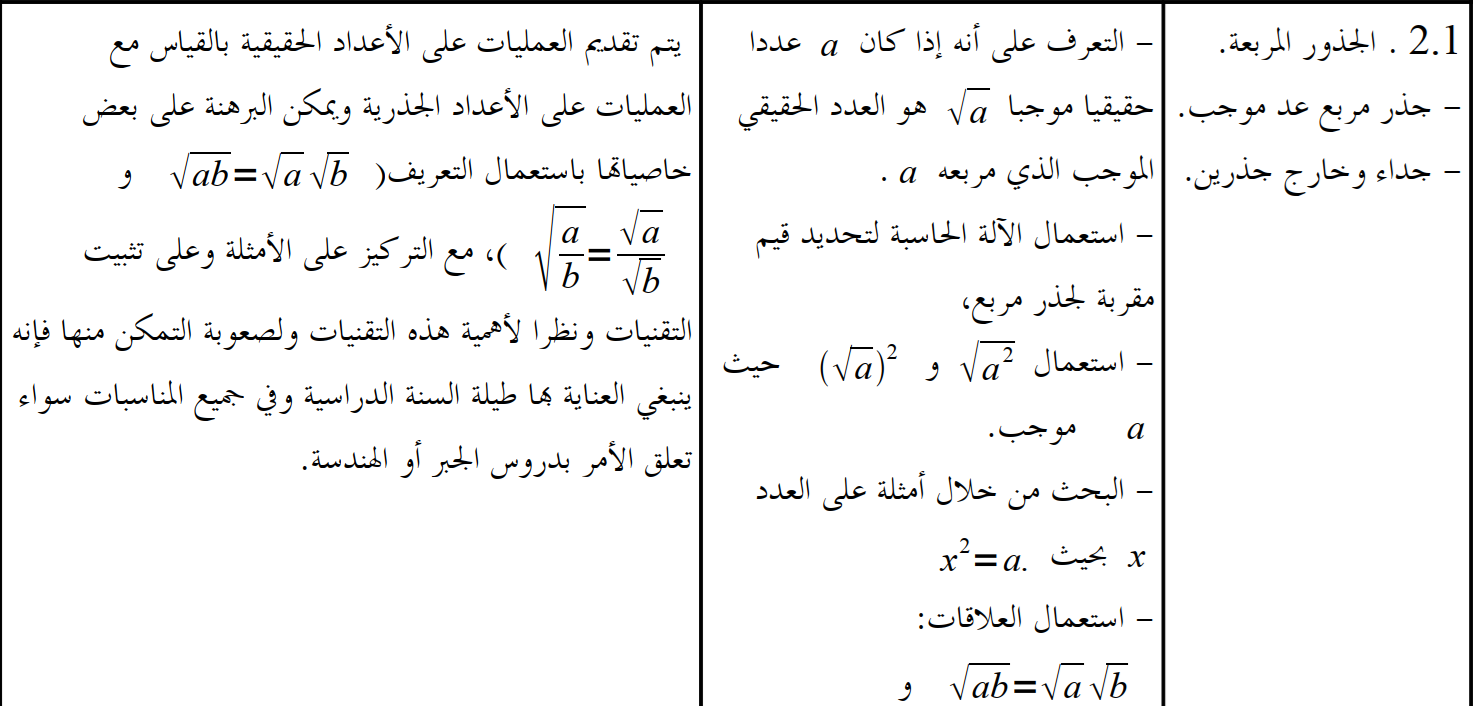
\includegraphics[width=\linewidth]{Les racines carrées.png}	
		\textcolor{black}{\myfont\bfseries Les pré-requis :} Le théorème de Pythagore, Les identités remarquables, Les équations, Les puissances, Développement et factorisation.
		\\
		\textcolor{black}{\myfont\bfseries Les outils utilisés  :} Livre scolaire, Les ressources, les instructions pédagogiques.
	\end{boxtwo}\newpage
	\renewcommand{\baselinestretch}{1.0}
	\begin{longtable}{|>{\centering\arraybackslash}p{3cm}|>{\raggedright\arraybackslash}p{5cm}|>{\raggedright\arraybackslash}p{13.5cm}|>{\raggedright\arraybackslash}p{5cm}|}
		\hline
		\rowcolor{black!20!white}\sffamily\textbf{OBJECTIFS}  &\sffamily\centering \textbf{ACTIVITÉS}
		& \sffamily\centering \textbf{CONTENU DE COURS} & \sffamily \textbf{APPLICATIONS}\\
		\hline 
		
		& \colorbox{yellow!50!white}{\uline{\sffamily \textbf{Activité-1 :} }}\par%\bigskip
		\textbf{1)} Quelle la longueur de la diagonale d'un carré dont le côté mesure 1m ?
		
		\textbf{2)} Quel est le nombre positif dont le carré est égale à 2 ?\vspace*{.3cm}
		
		\begin{tabular}{|c|c|c|c|c|}
			\hline
			\rule[-1ex]{0pt}{2.5ex} x & 1 & 2 & 1.5 & 1.42\\
			\hline
			\rule[-1ex]{0pt}{2.5ex} $x^2$ & 1 & 4 & 2.25 & 2.0164 \\
			\hline
		\end{tabular}
		\begin{tabular}{|c|c|}
			\hline
			\rule[-1ex]{0pt}{2.5ex} 1.41 & 1.415 \\
			\hline
			\rule[-1ex]{0pt}{2.5ex} 1.9881 & 2.002225 \\
			\hline
		\end{tabular}\vspace*{.3cm}
		
		Le nombre cherché n'a pas d'écriture décimale, et n'est pas un nombre rationnel. Ainsi, on a défini ce nombre à l'aide d'une écriture nouvelle: $\mathbf{\sqrt{2}}$
		
		\textbf{3)} Complète par le nombre qui convient:
		$\left(...\right)^2 = 25$ ; $\left(...\right)^2 = 36$ ; $\left(...\right)^2 = 121$
		
		\textbf{4)} Complète :\vspace*{.3cm}
		
		\begin{tabular}[width=5cm]{|c|c|c|c|c|}
			\hline
			\rule[-1ex]{0pt}{2.5ex} x & 4 & 3 & 7 & 9 \\
			\hline
			\rule[-1ex]{0pt}{2.5ex} $x^{2}$ & \textcolor{white}{....} & \textcolor{white}{....} & \textcolor{white}{....} & \textcolor{white}{....} \\
			\hline
			\rule[-1ex]{0pt}{2.5ex} $\sqrt{x^{2}}$ & \textcolor{white}{....} & \textcolor{white}{....} & \textcolor{white}{....} & \textcolor{white}{....} \\
			\hline
		\end{tabular}
		\vspace*{.3cm}
		
		Que remarquer vous?
		
		& 
		%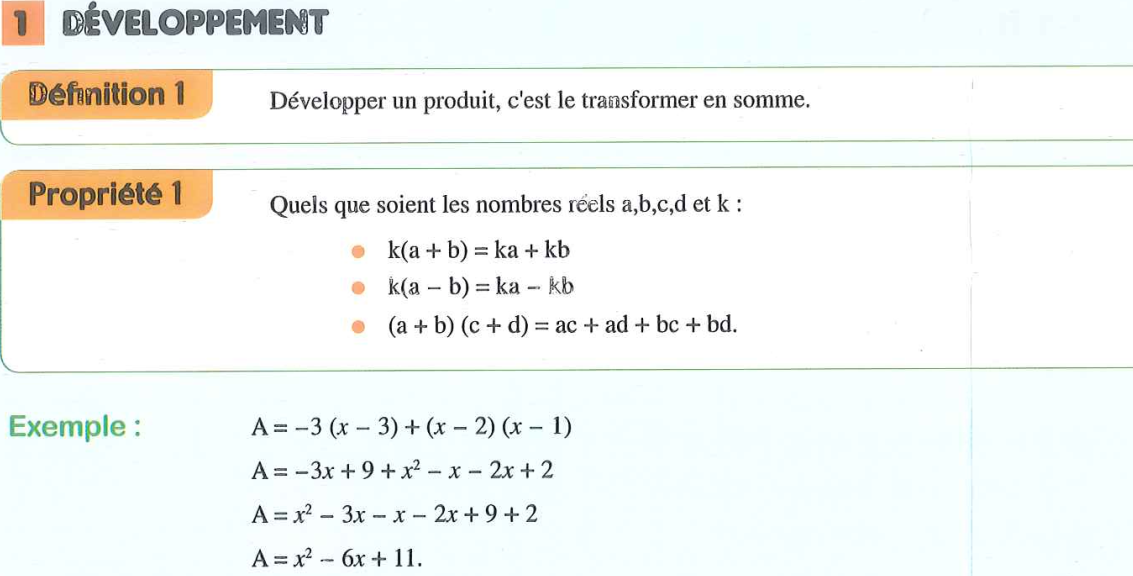
\includegraphics[width=\linewidth]{1.png}	
		\textcolor{Red}{\uline{\sffamily \textbf{I. La racine carrée d'un nombre réel positif :} }}\par
		%\textcolor{Green}{\uline{\sffamily \textbf{1) Définition:} }}\par
		\begin{BoxRafa}[colbacktitle = green]{Définition}
			Soit $a$ un nombre réel positif.
			\underline{\textbf{La racine carrée}} de $a$ est le nombre  \textcolor{Green}{\textbf{réel positif}} dont le carré est égale à $a$.
			
			\textbf{La racine carrée} de $a$ se note: $\mathbf{\sqrt{a}}$ et on a : \underline{$\mathbf{\sqrt{a^2} = a}$}
		\end{BoxRafa}
		\colorbox{yellow!50!white}{\uline{\sffamily \textbf{Autrement dit :}}}\par
			a un nombre réel positif et b un nombre réel positif. \underline{\textbf{si $\mathbf{a = b^2}$ alors $\mathbf{\sqrt{a} = b}$}}
		
		\colorbox{Gray!50!white}{\uline{\sffamily \textbf{Exemples}}}\par
		
		\begin{tabularx}{13.5cm}{X|X|X|X}
%			\hline
%			\rule[-1ex]{0pt}{2.5ex}
			 $\sqrt{0} = 0$ & $\left(\sqrt{3}\right)^2 = 3$ & $\sqrt{16}=\sqrt{4^2}$ & $\sqrt{1.21}=\sqrt{\left(1.1\right)^2}$\\
%			\hline
%			\rule[-1ex]{0pt}{2.5ex} 
			$\sqrt{1} = 1$ & $\left(\sqrt{5}\right)^2 = 5$ & $\qquad= 4$ & $\qquad\quad= 1.1$ \\
%			\hline
		\end{tabularx}
		
		& \colorbox{yellow!50!white}{\uline{\sffamily \textbf{Exercice-1:} }}\par
		Calculer :
		
		$\begin{aligned}
			&A=\sqrt{16} \\
			&B=\sqrt{9} \\
			&C=5\sqrt{100} \\
			&D=\dfrac{4}{\sqrt{100}} \\
			&E=\dfrac{\sqrt{81}}{\sqrt{25}} \\
			&F=\sqrt{25}+3\sqrt{49}
		\end{aligned}$
		\\ \hline
		&	
		\colorbox{Orange!50!white}{\uline{\sffamily \textbf{Activité-2 :}}}\par
		\textbf{1)} Complète le tableau:\vspace*{-.3cm}
		
		\hspace*{2.5cm}
			\begin{rotate}{-90}
				\begin{tabular}{|c|c|c|c|c|c|c|}
					\hline
					\rule[-2ex]{0pt}{5ex} a & b & $\sqrt{a}$ & $\sqrt{b}$ & $a\times b$ & $\sqrt{a\times b}$ & $\sqrt{a}\times\sqrt{b}$\\
					\hline
					\rule[-2ex]{0pt}{5ex} 9 & 16 &  & &  & & \\
					\hline
					\rule[-2ex]{0pt}{5ex} 25 & 4 &  &  &  & &  \\
					\hline
					\rule[-2ex]{0pt}{5ex} 36 & 64 &  &  &  & &  \\
					\hline
					\rule[-2ex]{0pt}{5ex} 49 & 81 &  &  &  & &  \\
					\hline
				\end{tabular}
			\end{rotate}.
		\vspace*{9cm}	
		
		Que peut-on déduire?
		
		\textbf{2)} Calculer:
		
		$\sqrt{9}+\sqrt{16}$ et $\sqrt{9+16}$
		
		Que remarque-vous?
			&
		\textcolor{Red}{\uline{\sffamily \textbf{II. Les opérations sur les racines carrées.:}}}\par
		\textcolor{Green}{\uline{\sffamily \textbf{1)La racine carrée et produit:}}}\par
		
		\begin{BoxRafa}[colbacktitle = green]{Propriété}
			$a$ et $b$ deux nombres réels positifs. Alors:  \tcbhighmath[boxrule=0.3pt,colframe=red,drop fuzzy shadow=red]{\mathbf{\sqrt{a\times b}=\sqrt{a}\times\sqrt{b}}}
		\end{BoxRafa}
		\begin{BoxRafa}[colbacktitle = green]{Résultat}
			$a$ et $b$ deux nombres réels positifs. Alors: 
			
			 \hspace*{4cm}\tcbhighmath[boxrule=0.3pt,colframe=red,drop fuzzy shadow=red]{\mathbf{\sqrt{a^2\times b}=\sqrt{a^2}\times\sqrt{b}}}
			
			\hspace*{5.5cm}\tcbhighmath[boxrule=0.3pt,colframe=red,drop fuzzy shadow=red]{\mathbf{=a\times\sqrt{b}}}
			
			\hspace*{5.5cm}\tcbhighmath[boxrule=0.3pt,colframe=red,drop fuzzy shadow=red]{\mathbf{=a\sqrt{b}}}
		\end{BoxRafa}
		\begin{BoxRafa}[colbacktitle = Orange]{Exemples-1:}
			
			$\begin{aligned}
				&\sqrt{80}&\qquad\qquad\qquad\qquad\qquad\qquad|\quad&\sqrt{3}\times\sqrt{7}=\sqrt{3\times7}\\
				&=\sqrt{16}\times\sqrt{5}&\qquad\qquad\qquad\qquad\qquad\qquad|\quad&=\sqrt{21}\\
				&=\sqrt{4^2}\times\sqrt{5}&\qquad\qquad\qquad\qquad\qquad\qquad|\quad&\\
				&=4\times\sqrt{5}&\qquad\qquad\qquad\qquad\qquad\qquad|\quad&\sqrt{2}\times\sqrt{4}\times\sqrt{3}=\sqrt{2\times3\times4}\\
				&=4\sqrt{5}&\qquad\qquad\qquad\qquad\qquad\qquad|\quad&=\sqrt{24}\\
			\end{aligned}$
			
		\end{BoxRafa}
		& \colorbox{yellow!50!white}{\uline{\sffamily \textbf{Exercice-2:} }}\par
		Réduire les expressions suivantes :
		
		$\begin{aligned}
			&A=\sqrt{2}\times\sqrt{32} \\
			&B=\sqrt{75} \\
			&C=\sqrt{27} \\
			&D=\sqrt{48} \\
			&E=\sqrt{56} \\
			&F=\sqrt{242}
		\end{aligned}$
		\\ \hline
		
		Découvrir la relation $\sqrt{\dfrac{a}{b}}=\dfrac{\sqrt{a}}{\sqrt{b}}$ &	
		\colorbox{Orange!50!white}{\uline{\sffamily \textbf{Activité-3 :}}}\par
		\textbf{1)} Complète le tableau:\vspace*{-.3cm}
		
		\hspace*{2.5cm}
		\begin{rotate}{-90}
			\begin{tabular}{|c|c|c|c|c|c|c|}
				\hline
				\rule[-2ex]{0pt}{5ex} a & b & $\sqrt{a}$ & $\sqrt{b}$ & $\dfrac{a}{b}$ & $\sqrt{\dfrac{a}{b}}$ & $\dfrac{\sqrt{a}}{\sqrt{b}}$\\
				\hline
				\rule[-2ex]{0pt}{5ex} 9 & 16 &  & &  & & \\
				\hline
				\rule[-2ex]{0pt}{5ex} 25 & 4 &  &  &  & &  \\
				\hline
				\rule[-2ex]{0pt}{5ex} 36 & 64 &  &  &  & &  \\
				\hline
				\rule[-2ex]{0pt}{5ex} 49 & 81 &  &  &  & &  \\
				\hline
			\end{tabular}
		\end{rotate}.
		\vspace*{7cm}	
		
		Que peut-on déduire?
		
		& 	
%		\textcolor{Red}{\uline{\sffamily \textbf{III. Identités remarquables:} }}\par
		\textcolor{Green}{\uline{\sffamily \textbf{2) La racine carrée et quotient:} }}\par
		\begin{BoxRafa}[colbacktitle = green]{Propriété}
			$a$ et $b$ deux nombres réels positifs et $b\neq0$.
			$$\mathbf{\sqrt{\dfrac{a}{b}}=\dfrac{\sqrt{a}}{\sqrt{b}}}$$
		\end{BoxRafa}
		\begin{BoxRafa}[colbacktitle = Orange]{Exemples-1:}
			
			$\begin{aligned}
				&\dfrac{\sqrt{55}}{\sqrt{45}}=\sqrt{\dfrac{55}{45}}&\qquad\qquad\qquad\qquad\qquad\qquad|\quad&\sqrt{\dfrac{9}{16}}=\dfrac{\sqrt{9}}{\sqrt{16}}\\
				&\qquad=\sqrt{\dfrac{5\times11}{5\times9}}&\qquad\qquad\qquad\qquad\qquad\qquad|\quad&\qquad=\dfrac{\sqrt{3^2}}{\sqrt{4^2}}\\
				&\qquad=\sqrt{\dfrac{11}{9}}&\qquad\qquad\qquad\qquad\qquad\qquad|\quad&\qquad=\dfrac{3}{4}\\
			\end{aligned}$
			
		\end{BoxRafa}&
		\colorbox{yellow!50!white}{\uline{\sffamily \textbf{Exercice-3:}}}\par
		Réduire les expressions suivantes :
		
		$\begin{aligned}
			&A=\dfrac{\sqrt{4}}{\sqrt{81}}&\qquad&B=\sqrt{\dfrac{8}{18}} \\ &C=\sqrt{\dfrac{3}{16}}&\qquad&D=\dfrac{\sqrt{9}}{\sqrt{7}}\times\sqrt{7}
		\end{aligned}$
		
		\\
		\hline
		Éliminer la racine carrée d'un dénominateur
		&
		\colorbox{yellow!50!white}{\uline{\sffamily \textbf{Activité-4 :} }}\par%\bigskip
		$a$ et $b$ deux nombres réels positifs
		
		1) Montrer que:
		$$(\sqrt{a}-\sqrt{b})(\sqrt{a}+\sqrt{b})=a-b$$
		On considère que : $a \neq 0$ et $b \neq 0$.
		
		2) Montrer que: $\dfrac {1}{\sqrt {a}}= \dfrac{\sqrt {a}}{a}.$
		
		3) Montrer que:
		$$\dfrac1{\sqrt{a}-\sqrt{b}}=\dfrac{\sqrt{a}+\sqrt{b}}{a-b}$$
		
		&
		\textcolor{Green}{\uline{\sffamily \textbf{3) Éliminer la racine carrée au dénominateur:} }}\par
		\begin{BoxRafa}[colbacktitle = green]{Propriété}
			$a$ un nombre réel positif et $a\neq0$.%$$\mathbf{\dfrac{1}{\sqrt{a}}=\dfrac{\sqrt{a}}{a}}$$
			
			\qquad\qquad\qquad\qquad\qquad\qquad\qquad\begin{tikzpicture}[
				squarednode/.style={rectangle, draw=red!60, fill=red!5, very thick, minimum size=5mm},
				]
				%Nodes
				\node[squarednode]      (maintopic)                              {$\mathbf{\dfrac{1}{\sqrt{a}}=\dfrac{\sqrt{a}}{a}}$};
			\end{tikzpicture}
		\end{BoxRafa}
		\begin{BoxRafa}[colbacktitle = Orange]{Remarque:}
			
			\qquad\qquad\qquad\qquad\begin{tikzpicture}[
				squarednode/.style={rectangle, draw=red!60, fill=red!5, very thick, minimum size=5mm},
				]
				%Nodes
				\node[squarednode]      (maintopic)                              {$\mathbf{\dfrac{1}{\sqrt{a}}=\dfrac{1\times\sqrt{a}}{\sqrt{a}\times\sqrt{a}}=\dfrac{\sqrt{a}}{\left(\sqrt{a}\right)^{2}}=\dfrac{\sqrt{a}}{a}}$};
			\end{tikzpicture}
		\end{BoxRafa}
		\begin{BoxRafa}[colbacktitle = Orange]{Exemples-1:}
			
			$$\begin{aligned}
				\dfrac{5}{\sqrt{3}} =\dfrac{5\times\sqrt3}{\sqrt3\times\sqrt3} 
				=\dfrac{5\sqrt3}{\left(\sqrt3\right)^2}
				=\dfrac{5\sqrt{3}}{3} 
			\end{aligned}$$
			
		\end{BoxRafa}
		\begin{BoxRafa}[colbacktitle = green]{Propriété}
			$a$ et $b$ deux nombres réels positifs avec $a\neq0$ et $b\neq0$.
			
			\qquad\qquad\qquad\qquad\qquad\qquad\qquad\begin{tikzpicture}[
				squarednode/.style={rectangle, draw=red!60, fill=red!5, very thick, minimum size=5mm},
				]
				%Nodes
				\node[squarednode]      (maintopic)                              {$\mathbf{\dfrac1{\sqrt{a}-\sqrt{b}}=\dfrac{\sqrt{a}+\sqrt{b}}{a-b}}$};
			\end{tikzpicture}
		\end{BoxRafa}
		\begin{BoxRafa}[colbacktitle = Orange]{Exemples-1:}
		
		$$\begin{aligned}
			\dfrac{2}{1-\sqrt{5}}=\frac{2\times(1+\sqrt{5})}{(1-\sqrt{5})(1+\sqrt{5})} 
			=\dfrac{2(1+\sqrt{5})}{1^{2}-\left(\sqrt{5}\right)^{2}} 
			=\dfrac{2(1+\sqrt{5})}{1-5} 
			=\dfrac{2(1+\sqrt{5})}{-4}
%			=\dfrac{-(1+\sqrt{5})}{2}  
		\end{aligned}$$
		
		\textcolor{Green}{\uline{\sffamily \textbf{Remarque} }}\par
		Le conjugué de $1-\sqrt{5}$ est $1+\sqrt{5}$
		\end{BoxRafa}
		&
		\colorbox{yellow!50!white}{\uline{\sffamily \textbf{Exercice-4:}}}\par
		Supprimer la racine carrée au dénominateur dans :
		
		1) $$\dfrac{2}{\sqrt{5}}$$

		2) $$\dfrac{\sqrt{3}}{5\sqrt{2}}$$
		
		3) $$\dfrac{2+\sqrt{5}}{7\sqrt{3}}$$
		
		4) $$\dfrac{5}{\sqrt{7}-\sqrt{3}}$$
		
		\colorbox{yellow!50!white}{\uline{\sffamily \textbf{Exercice-5:}}}\par
		1) Supprimer la racine carrée au dénominateur.
		$$\begin{aligned}
			&A=\dfrac{3}{\sqrt{11}}\quad;\quad B=\dfrac{11}{2\sqrt{5}}\\
			&C=\dfrac{2\sqrt{3}}{5\sqrt{5}}\quad;\quad D=\dfrac{1}{\sqrt{3}+1}\\
			&E=\dfrac{2\sqrt{7}}{\sqrt{10}-\sqrt{7}} \\
		\end{aligned}$$
		
		\\ \hline Résolution de l'équation de la forme $x^2=a$
		&	
		\colorbox{yellow!50!white}{\uline{\sffamily \textbf{Activité-5 :} }}\par%\bigskip
		
		1) Résoudre les équations suivantes:
		$$\begin{aligned}
			&x^{2}=9\quad;\quad x^{2}=4\\
			&x^{2}=6\quad;\quad x^{2}=0\\
			&x^{2}=5\quad;\quad x^{2}=-1
		\end{aligned}$$
		& 	
%		\textcolor{Red}{\uline{\sffamily \textbf{}}}\par
		\textcolor{Green}{\uline{\sffamily \textbf{4) Résoudre une équation de la forme $x^2= a$: }}}\par
		\begin{BoxRafa}[colbacktitle = green]{Règle :1}
			Soit $a$ un nombre réel alors:
			\begin{itemize}
				\item[$\blacktriangleright$]  Si \underline{$\mathbf{a> 0}$}, alors l'équation \underline{$x^2= a$} admet deux solutions: $\mathbf{\sqrt{a}}$ et $\mathbf{-\sqrt a}$.
				\item[$\blacktriangleright$]  Si \underline{$\mathbf{a=0}$},alors l'équation \underline{$x^2=a$} admet une \underline{unique solution: $0$}.
				\item[$\blacktriangleright$]  Si $a< 0$, alors l'équation \textbf{n'admet aucune solution}.
			\end{itemize}
		\end{BoxRafa}
		\begin{BoxRafa}[colbacktitle = Orange]{Exemples:}
			
			\begin{itemize}
				\item[$\blacksquare$]  Si \underline{$\mathbf{a> 0}$}, alors l'équation \underline{$x^2= a$} admet deux solutions: $\mathbf{\sqrt{a}}$ et $\mathbf{-\sqrt a}$.
				\item[$\blacktriangleright$]  Si \underline{$\mathbf{a=0}$},alors l'équation \underline{$x^2=a$} admet une \underline{unique solution: $0$}.
			\end{itemize}
			
		\end{BoxRafa}
		\begin{BoxRafa}[colbacktitle = Orange]{Exemples:}
			
			\begin{itemize}
				\item[$\blacksquare$] \underline{Resoudre l'equation suivante: ${x}^{2}=7$}
				
				on a: $x^{2}= 7$
				
				et comme $7>0$ alors l'équation admet deux solutions: $\sqrt{7}$ et $-\sqrt{7}$
				
				\item[$\blacksquare$] \underline{Resoudre l'equation suivante: $x^2= - 2$}
				
				on a: $x^{2}= - 2$
				
				et comme $-2<0$ alors l'équation n'admet pas de solutions.
			\end{itemize}
			
		\end{BoxRafa}
		
		&
		\colorbox{yellow!50!white}{\uline{\sffamily \textbf{Exercice-6:}}}\par
		Résoudre les équations suivantes :
		$$x^{2}=11\quad;\quad x^{2}+3=0$$
		$$x^{2}-25=0\quad;\quad x^{2}=121$$
		$$\dfrac{x^2}4=5$$
		\\
		\hline
		&	
		\colorbox{yellow!50!white}{\uline{\sffamily \textbf{Activité-6 :} }}\par%\bigskip
		
		Simplifier les expressions suivantes : 
		
		$\begin{aligned}
			&A=\left(\sqrt{2}\right)^{3}\times\left(\sqrt{2}\right)^{5}\times\left(\sqrt{2}\right) \\
			&B=\left(\sqrt{3}\right)^{-3}\times\left(\sqrt{3}\right)^{5} \\
			&C=\left(\sqrt{3}\right)^{2}\times5^{2} \\
			&D=\left(\left(\sqrt{3}\right)^{2}\right)^{3} \\
			&E=\frac{\left(\sqrt{3}\right)^{5}}{\left(\sqrt{3}\right)^{3}}
		\end{aligned}$
		& 	
		\textcolor{Red}{\uline{\sffamily \textbf{V. Propriétés des puissances} }}\par
		%\textcolor{Green}{\uline{\sffamily \textbf{1) Carré d'une somme:} }}\par
		{Les puissances ont des propriétés spécifiques permettant des calculs rapides.}
		\begin{BoxRafa}[colbacktitle = green]{RÈGLE N$^\circ$1:(Produit De Deux Puissances)}
			\hspace*{2cm}\begin{tikzpicture}[
				roundnode/.style={circle, draw=green!60, fill=green!5, very thick, minimum size=7mm},
				squarednode/.style={rectangle, draw=red!60, fill=red!5, very thick, minimum size=5mm},
				]
				%Nodes
				\node[squarednode]	(maintopic)	{$\underbrace{\qquad a^m\times a^p\qquad}_{\text{C'est le même nombre}}=\underbrace{\quad\qquad a^{m+p}\quad\qquad}_{\text{On additionne les puissances}}$};
				%\node[roundnode]        (uppercircle)       [right=of maintopic] {=};
				%\node[squarednode]      (rightsquare)       [right=of uppercircle] {$a^2+2ab+b^2$};
				%\node[roundnode]        (lowercircle)       [below=of maintopic] {4};
				
				%Lines
				%\draw[->] (uppercircle.south) -- (maintopic.north);
				%\draw[->] (maintopic.north) .. controls +(up:7mm) and +(right:0mm) .. (rightsquare.north);
				%\draw[->] (rightsquare.south) .. controls +(down:7mm) and +(right:0mm) .. (maintopic.south);
				%\draw[->] (rightsquare.south) .. controls +(down:7mm) and +(right:7mm) .. (lowercircle.east);
			\end{tikzpicture}\vspace{-.1cm}
		\end{BoxRafa}
		
		\begin{BoxRafa}[colbacktitle = Orange]{Exemples:}
			
			\textbf{Calculons les nombres $x=\frac{5^8}{5^6}$ et $y=\frac{3^{14}}{3^8}$ en donnant les résultats sous forme de puissances.}
			
			On applique directement la règle qui nous donne : $x=3^{4}\times3^{2}=\underbrace{\qquad\qquad 3^{4+2}\qquad\qquad}_{\text{On additionne les puissances}}=3^{6}$ et de même $y=7^3\times7^2=7^{3+2}=7^5$
			
		\end{BoxRafa}
		\begin{BoxRafa}[colbacktitle = green]{RÈGLE N$^\circ$2:(Quotient De Deux Puissances)}
			\hspace*{1.5cm}\begin{tikzpicture}[
				roundnode/.style={circle, draw=green!60, fill=green!5, very thick, minimum size=7mm},
				squarednode/.style={rectangle, draw=red!60, fill=red!5, very thick, minimum size=5mm},
				]
				%Nodes
				\node[squarednode]	(maintopic)	{$\underbrace{\qquad\qquad\frac{a^m}{a^p}\qquad\qquad}_{\text{C'est le même nombre }a}=\underbrace{\qquad\qquad a^{m-p}\qquad\qquad}_{\text{On soustrait les puissances}}$};
				%\node[roundnode]        (uppercircle)       [right=of maintopic] {=};
				%\node[squarednode]      (rightsquare)       [right=of uppercircle] {$a^2+2ab+b^2$};
				%\node[roundnode]        (lowercircle)       [below=of maintopic] {4};
				
				%Lines
				%\draw[->] (uppercircle.south) -- (maintopic.north);
				%\draw[->] (maintopic.north) .. controls +(up:7mm) and +(right:0mm) .. (rightsquare.north);
				%\draw[->] (rightsquare.south) .. controls +(down:7mm) and +(right:0mm) .. (maintopic.south);
				%\draw[->] (rightsquare.south) .. controls +(down:7mm) and +(right:7mm) .. (lowercircle.east);
			\end{tikzpicture}\vspace{-.1cm}
		\end{BoxRafa}
		
		\begin{BoxRafa}[colbacktitle = Orange]{Exemples:}
			\textbf{Calculons les nombres $x=3^4\times3^2$ et $y=7^{3}\times7^{2}$ en donnant les résultats sous forme de puissances.}
			
			La règle nous donne directement: $x=\frac{5^{8}}{5^{6}}=\underbrace{\quad\qquad5^{8-6}\quad\qquad}_{\text{On soustrait les puissances}}=5^{2}$ 
			
			Et de même $y=\frac{3^{14}}{3^8}=3^{14-8}=3^6$
			
		\end{BoxRafa}
		
		&
		\colorbox{yellow!50!white}{\uline{\sffamily \textbf{Exercice-8:}}}\par
		Simplifier les expressions suivantes :
		
		$\begin{aligned}&\left(\sqrt{7}\right)^{-13}\times\left(\sqrt{7}\right)^{65}\\&\left(\sqrt{3}\right)^{6}\times\left(\sqrt{3}\right)^{-5}\times\left(\sqrt{3}\right)\end{aligned}$
		\colorbox{yellow!50!white}{\uline{\sffamily \textbf{Exercice-9:}}}\par
		Simplifier les expressions suivantes :
		
		$\begin{aligned}
			&a= (-4)^{3}\times(-4)^{12} \\
			&b=5^{6}\times(\sqrt{2})^{6}  \\
			&c= \frac{(-\sqrt{2})^{3}}{(-\sqrt{2})^{-8}} \\
			&d=\left(\sqrt{2}^{5}\right)^{-2}  \\
			&e= 5^{-3}\times3\times(5^{2})^{7}\times9^{5}  \\
			&f= \frac{(-21)^{3}\times5}{35^{3}\times3}  \\
			&j= \frac{\mathrm{a^{2}b(a^{-1}\times b^{2})^{-3}}}{\mathrm{a(a^{2}\times b)^{5}(b^{2})^{-1}}} 
		\end{aligned}$
		\\
		\hline
	\end{longtable}
\end{document}